\documentclass[11pt]{article}
\usepackage{geometry}                
\geometry{letterpaper}                 
\usepackage[parfill]{parskip}        
\usepackage{graphicx}
\usepackage{amssymb}
\usepackage{amsmath}
\usepackage{epstopdf}
\usepackage{verbatim}
\usepackage{float}
\usepackage[T1]{fontenc}
\DeclareGraphicsRule{.tif}{png}{.png}{`convert #1 `dirname #1`/`basename #1 .tif`.png}
\usepackage{color}
\usepackage{textcomp}
\definecolor{listinggray}{gray}{0.9}



\begin{document}

\section*{Review of 216 Topics, 10/24/13}
Mai Le

If you haven't taken EECS 216, and you're wondering what you missed out on, don't worry- a lot of that stuff is not relevant to us here in EECS 451. Here I'll recap just the material from 216 that directly connects to our class. You will not be held responsible for this supplementary material (e.g. on an exam), but it can help you better understand a lot of the concepts in this class. 

\section{Continuous Time Signals}

A continuous time signal is defined over all real values (usually the domain is $t$ for "time", but it can be defined over other physical quantities as well). The notation looks like $x(t)$.

Some examples you've already seen:

\begin{description}
	\item[Dirac delta] $\delta(t)$ 
	
	\qquad For more info about the Dirac delta (including its sifting and sampling properties), please see handout from Disc 1.
	\item[Dirac comb]  $s(t) = \sum\limits_{n=-\infty}^\infty \delta(t-nT)$
	
	\qquad (also known as a train of impulses or a Shah function (from the Cyrillic symbol))
	\item[Cosine] (example from class) $x_c(t) = cos(\Omega_0 t)$
\end{description}

Some other examples:

\begin{description}
	\item[Rect] $x(t) = \begin{cases} 1, & |t| <\frac{1}{2} \\
	0, & |t| > \frac{1}{2}
	\end{cases}$  (the value at $t=\pm \frac{1}{2}$ depends on which textbook you use)
	\item[Sinc] $sinc(t) = \frac{sin(\pi t)}{\pi t}$. 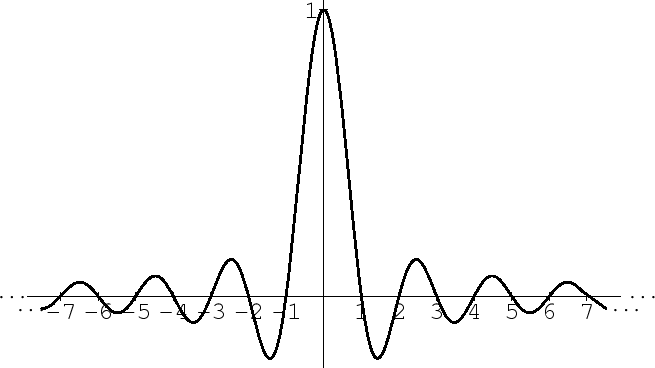
\includegraphics[scale=0.3]{sinc.png} 
\end{description}


\section{Continuous Time Fourier Transform}
As described in the table from Lecture 12, the Continuous Time Fourier Transform (CTFT) goes from a continuous time domain to a continuous frequency domain. The signal $x(t)$ does not need to be periodic to apply the CTFT (unlike the Continuous Time Fourier Series (CTFS) if you know about it). Unlike the DTFT from 451, the frequency domain is not periodic. For clarity, I'll denote this aperiodic frequency as $\tilde{\omega}$. Note: if you wish to refer to Wikipedia, this is the "non-unitary, angular frequency" version of the CTFT.

CTFT:
\[ X(\Omega) = \int_{-\infty}^\infty x(t) e^{-j \Omega t} dt
\]

inverse CTFT:
\[ x(t) = \frac{1}{2 \pi} \int_{-\infty}^\infty X(\Omega)e^{j \Omega t} d\Omega
\]

\subsection*{How do these formulas differ from the DTFT formulas? }
I list the following formulas for a discrete-signal $y[n]$ to differentiate from continuous-time $x(t)$. Remember, the DTFT does not apply to $x(t)$ and the CTFT does not apply to $y[n]$!

DTFT: $Y(w) = \sum_{n=-\infty}^\infty y[n] e^{-j \omega n}$.

IDTFT: $y[n] = \frac{1}{2 \pi} \int_{2\pi} Y(\omega)e^{j \omega n} d\omega$.
\begin{itemize}
	\item CTFT is an \textbf{integral} over $t$, not a \textbf{sum} over $n$.
	\item ICTFT is an integral over \textbf{all} $\Omega$, not just a period of $2 \pi$ in $\omega$, as in the IDTFT.
\end{itemize}

\subsection*{When do we use the CTFT compared to the DTFT (and the soon-to-be-learned DFT)?}
The CTFT is useful for theoretical analysis of many real world signals, because many real world signals are actually defined over a continuous domain. For example, a musical signal is actually over continuous time. It is only after sampling that it becomes a "discrete-time" signal. Later in this class you will learn about the DFT, which transforms between discrete time and discrete frequency. Most of modern signal processing is done through computers and thus focuses on digital (discrete-time and discrete-valued) signals and discrete transforms like the DFT, but continuous time analysis is still hugely important for theoretical analysis and  understanding of discrete time signals. 

\section{CTFT properties}

The CTFT shares a lot of properties of the DTFT, such as linearity, conjugation, time shifting, frequency shifting, Parseval's Theorem, differentiation, and integration. It also shares many symmetry properties. 

\subsection*{Convolution Theorem for CTFT}
Since the convolution theorem can be particularly useful, I'll rewrite it here for the CTFT:

\[
f(t) * g(t) \stackrel{CTFT}{\rightarrow } F(\Omega) G(\Omega) 
\]

\[
f(t)g(t) \stackrel{CTFT}{\rightarrow} \frac{1}{2\pi} F(\Omega) * G(\Omega)
\]

\subsection*{Duality}
A special property the CTFT does not share with the DTFT is duality. Because both the input and output domain are continuous, we can ask this question: what happens if you take the CTFT of a signal \textbf{twice}?

Let $X(\Omega)$ be the CTFT of $x(t)$. Though we usually only perform the CTFT on time signals to move them into the frequency domain, we can still apply the CTFT operator to it. Just think of the CTFT as some mathematical operator, devoid of time and frequency context. Then the output of the CTFT on $X(\Omega)$ is going to be back in the time domain, and in fact, it is $2\pi(-t)$!

\[ x(t) \stackrel{CTTF}{\rightarrow} X(\Omega) \stackrel{CTFT}{\rightarrow} 2\pi x(-t)
\]

Duality cannot exist for the DTFT because its input domain is discrete and its output domain is continuous, but we will see this duality property again with the DFT.

\section{Useful CTFT pairs to know}

Dirac comb $\rightarrow$ another Dirac comb! (Can you think of any other signals that stay the same, within some scaling or stretching factor, after the CTFT?)

\[
s(t) = \sum_{n=-\infty}^\infty \delta(t-nT) \leftrightarrow S(\Omega) = \frac{2 \pi}{T} \sum_{k=-\infty}^\infty \delta(\Omega - k\Omega_s),\ \Omega_s = \frac{2\pi}{T}
\]

1 $\rightarrow$ $\delta$

\[ 1 = 1(t) \leftrightarrow 2 \pi \delta(\Omega)
\]

Due to duality, we also have $\delta$ $\rightarrow$ 1

\[ \delta(t) \leftrightarrow 1 = 1(\Omega)
\]

Rect $\rightarrow$ sinc

\[ rect(t) \leftrightarrow sinc\left(\frac{\Omega} {2\pi}\right)
\]

Due to duality, we also have sinc $\rightarrow$ rect

\[ sinc(t) \leftrightarrow rect\left(\frac{\Omega}{2 \pi}\right)
\]

\section{Other Analogous Concepts}
If you are not familiar with these 216 concepts, don't fret. This is primarily to help people who have taken both classes see the connections between the courses. 

\begin{eqnarray*}
\text{\underline{continuous-time (CT)}} & & \text{\underline{discrete-time (DT)}}  \\
\text{Dirac delta} &\leftrightarrow& \text{Kronecker delta} \\
\text{Laplace Transform} &\leftrightarrow& \text{Z-Transform} \\
\text{continuous-time LTI system} &\leftrightarrow& \text{discrete-time LTI system} \\
\text{impulse response/transfer function of CT LTI system} &\leftrightarrow& \text{impulse response/transfer function of DT LTI system} \\
\text{CT Fourier Series} &\leftrightarrow& \text{DT Fourier Series} \\
&& \text{ and many more...}
\end{eqnarray*}
\end{document}